\documentclass[12pt, a4paper]{article}

% Text languages
\usepackage[spanish, english, UKenglish, USenglish, american, british]{babel}

% Accents
\usepackage[latin1]{inputenc}

% Maths
\usepackage{mathtools}
\usepackage{amsmath,amsthm,amssymb}

\DeclarePairedDelimiter\abs{\lvert}{\rvert}%
\DeclarePairedDelimiter\norm{\lVert}{\rVert}%

% Swap the definition of \abs* and \norm*, so that \abs
% and \norm resizes the size of the brackets, and the 
% starred version does not.
\makeatletter
\let\oldabs\abs
\def\abs{\@ifstar{\oldabs}{\oldabs*}}
%
\let\oldnorm\norm
\def\norm{\@ifstar{\oldnorm}{\oldnorm*}}
\makeatother


% https://www.overleaf.com/learn/latex/Page_size_and_margins
\usepackage{geometry}
\topmargin = -23pt
\oddsidemargin = 13pt
\headheight = 12pt
\headsep = 25pt
\textheight = 674pt
\textwidth = 426pt
\marginparsep = 10pt
\marginparwidth = 50pt
\footskip = 30pt
\marginparpush = 5pt
\hoffset = 0pt
\voffset = 0pt
\paperwidth = 597pt
\paperheight = 845pt

% Hyperlinks
\usepackage{hyperref}

% Figure
\usepackage{graphicx}
% \usepackage{subcaption}
\usepackage{etoc}
% Example
\newtheorem{exmp}{Example}[section]
% Algorithms
%\usepackage[]{algorithm2e}
%\usepackage{algorithm}% http://ctan.org/pkg/algorithm
%\usepackage{algpseudocode}% http://ctan.org/pkg/algorithmicx
\usepackage{algpseudocode}

\renewcommand{\thefootnote}{\arabic{footnote}} % 1, 2, 3... (la que hay por defecto)

\usepackage{titlesec}
\setcounter{secnumdepth}{5}

\titleformat{\paragraph}
{\normalfont\normalsize\bfseries}{\theparagraph}{1em}{}
\titlespacing*{\paragraph}
{0pt}{3.25ex plus 1ex minus .2ex}{1.5ex plus .2ex}

\usepackage{float}
%--------------------------------------------------------------------------
\title{Detection of/between similarity of documents with hashing}
\author{Roger Vilaseca Darn�, Xavier Lacasa Curto and Xavier Mart�n Ballesteros\\
  \small Algorithms\\
}
\date{1st December 2018}

\begin{document}
% Images
\graphicspath{ {./images/}, {./plots/} }

%\maketitle

\begin{titlepage}
	\centering
	{\scshape\LARGE UNIVERSITAT POLIT�CNICA DE CATALUNYA \par}
	\vspace{1cm}
	{\scshape\Large VISI� PER COMPUTADOR\par}
	\vspace{1.5cm}
	{\huge\bfseries Reconeixement autom�tic de flors\par}
	\vspace{2cm}
	{\Large\itshape Adri� Cabeza Sant'Anna i Xavier Mart�n Ballesteros\par}
	\vfill
	%\includegraphics[width=0.15\textwidth]{UPC.png}\par\vspace{1cm}
	%supervised by\par
	%Dr.~Mark \textsc{Brown}

	\vfill

% Bottom of the page
	{\large DATA}
\end{titlepage}

%\abstract{Esto es una plantilla simple para un articulo en \LaTeX.}

%	*********************** �NDEX *********************
%\setcounter{secnumdepth}{5}
%\setcounter{tocdepth}{5}

%\newpage
%  \tableofcontents
%\newpage

\section{Caracter�stiques extretes}

\subsection{Histograma del color}

\begin{figure}[H]
	\centering
	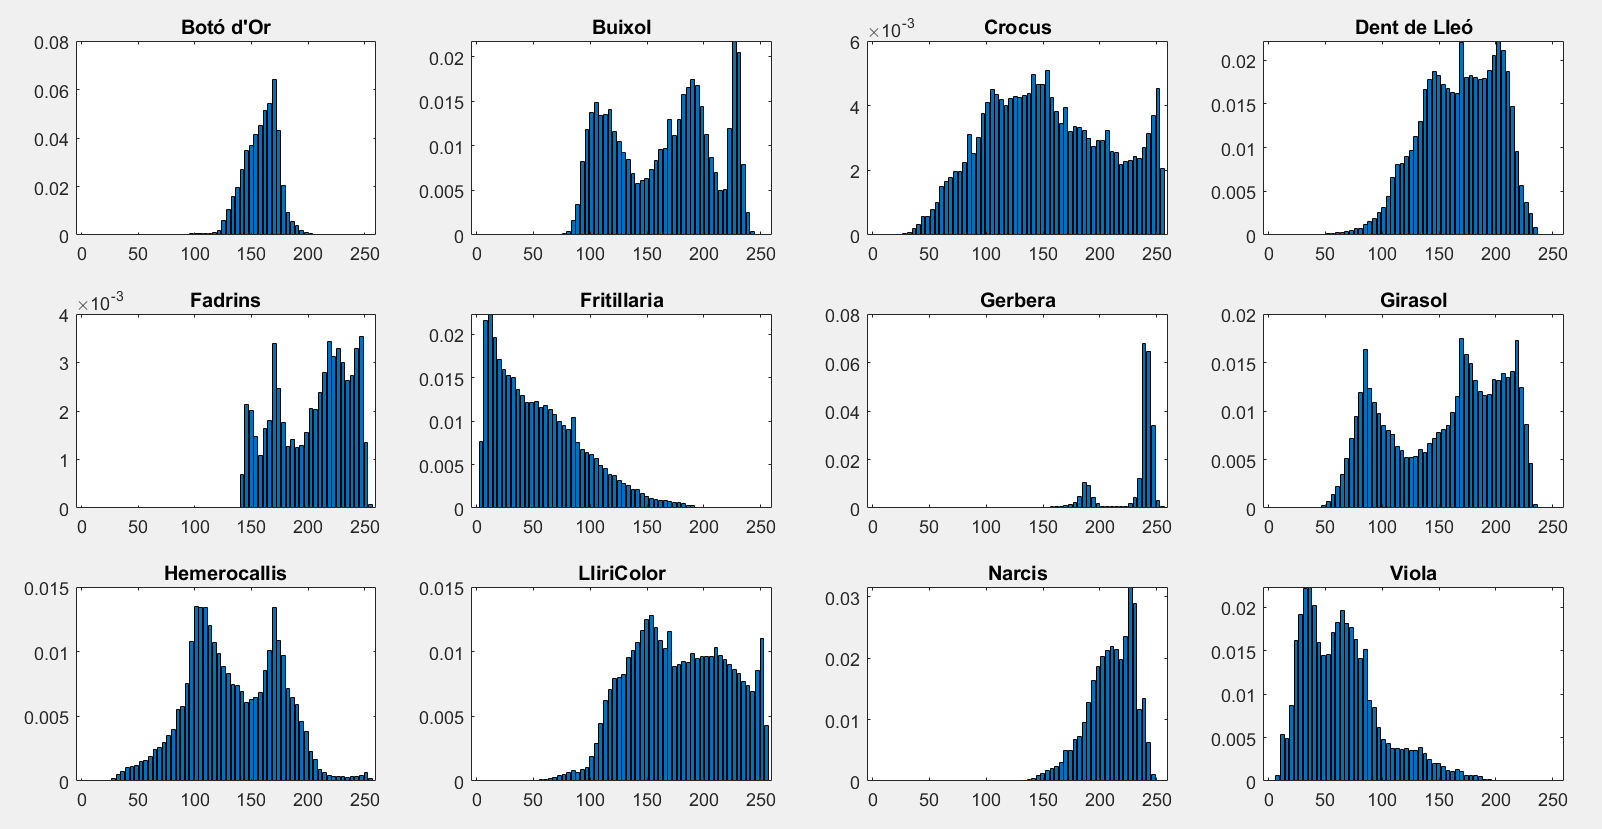
\includegraphics[scale=0.35]{./images/colorHistogram1}
	\caption{Prova1.}
\end{figure}

\begin{figure}[H]
	\centering
	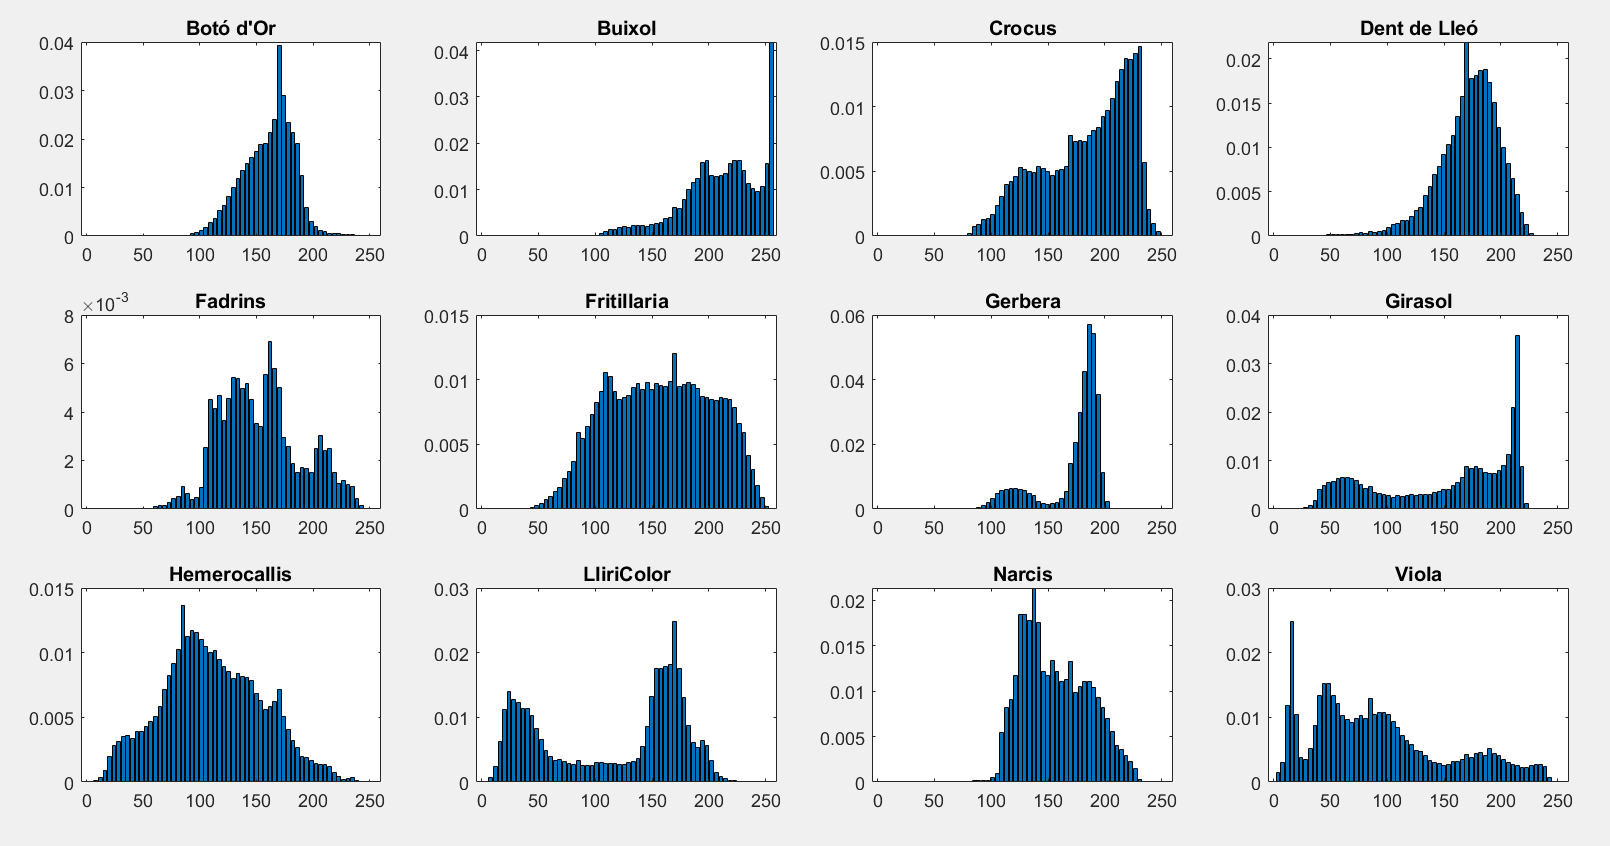
\includegraphics[scale=0.35]{./images/colorHistogram2}
	\caption{Prova2.}
\end{figure}

\begin{figure}[H]
	\centering
	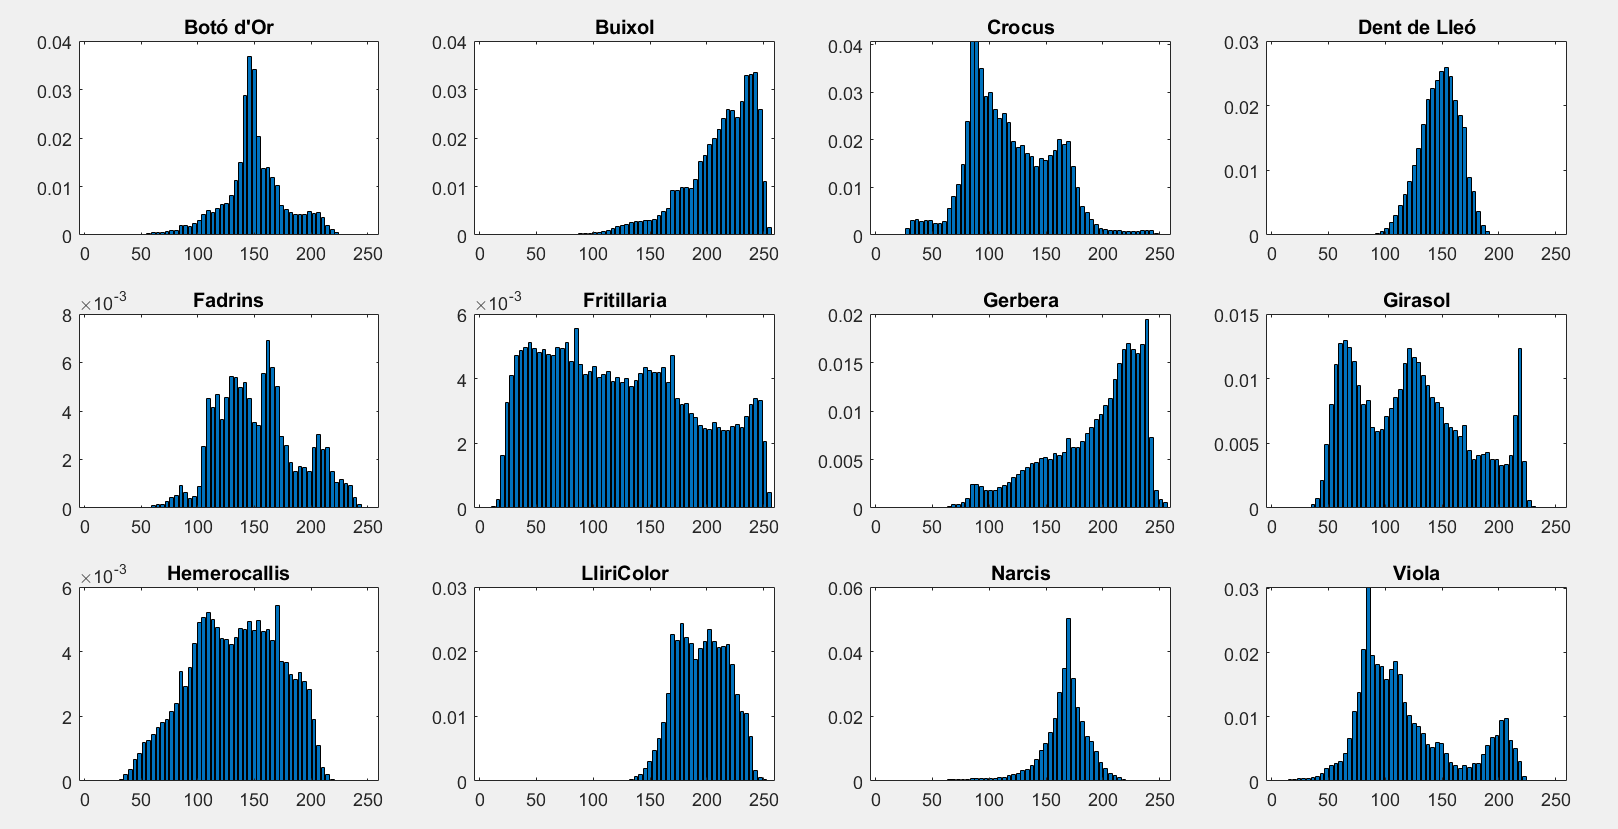
\includegraphics[scale=0.35]{./images/colorHistogram3}
	\caption{Prova3.}
\end{figure}


% Bibliograf�a.
%-----------------------------------------------------------------

\end{document}